\chapter{Process analysis}

Following the work of \cite{SegoviaHernandez2020}, let's analyse the esterification of lactic acid with methanol given by the following chemical reaction

\begin{equation}
	\underbrace{CH_3CHOHCOOH}_{Lactic~Acid} + \underbrace{CH_3OH}_{Methanol} \rightarrow \underbrace{CH_3CHOHCOOCH_3}_{Methyl~Lactate} + \underbrace{H_2O}_{Water}
\end{equation}

The reaction can autocatalyse using the acid for temperatures higher than approximately $340 K$. The kinetic model is used to represent the reaction rate, but the effect of the reverse reaction is neglected. Thus, the reaction rate is expressed as follows:

\begin{equation}
	r = k_1 \exp\left( \frac{-E_a}{RT} \right) a^2_{LACTIC} a_{MeOH}
\end{equation}

where $k_1$ is equal to $6.024 \times 10^8 ~[mol \cdot min^{-1}]$, $E_A$ is equal to $56.45~[kJ\cdot mol^{-1}]$, and $a_i$ is the activity of the component $i$.

\section{Initial simulation}

The thermodynamics is calculated based on the UNIFAC method. In statistical thermodynamics, the UNIFAC method (UNIQUAC Functional-group Activity Coefficients) is a semi-empirical system for predicting non-electrolyte activity in non-ideal mixtures. UNIFAC uses the functional groups present on the molecules that make up the liquid mixture to calculate activity coefficients. The activity of each of the solutions can be calculated by using interactions for each of the functional groups present on the molecules and some binary interaction coefficients. The UNIFAC correlation attempts to break down the problem of predicting interactions between molecules by describing molecular interactions based on the functional groups attached to the molecule. This is done in order to reduce the sheer number of binary interactions that would be needed to be measured to predict the state of the system.

In this case, $100~[kmol/h]$ of lactic acid is allowed to enter a tubular reactor. Methanol is also fed to the reactor, with a methanol/lactic acid mole ratio of $3:1$. The reactor operates at $340~[K]$ and $1~[bar]$. Esterification of lactic acid occurs inside the vessel; thus, the stream leaving the equipment contains methyl lactate, water, and unreacted methanol and lactic acid. The reaction occurs in a Plug Flow Reactor (PFR). The first parameter to be decided is the characteristic of the reactor, which in this case is set to \textit{reactor with specified temperature}, which means that the feed temperature determines the reactor's temperature. To set the initial simulation the reactor length is assumed to be $5~[m]$, and the diameter to be $0.1~[m]$. 

Because the kinetic model is provided as a power law, the reaction type is selected as \textit{POWERLAW}. The coefficients of the reactants (lactic acid and methanol) are set as -1, and the coefficients of the products (methyl lactate and water) are set as 1. The exponent is defined as 2 for lactic acid and 1 for methanol because it is the power for each component activity in the kinetic expression. The products are not involved in the kinetic model for the straight reaction. Thus, the field is left blank, which implies an exponent of 0. The values for the pre-exponential factor $k_1$ and the activation energy $E_a$ are known. The reference temperature $T_0$ is not specified; the exponent n is set as 0 to allow temperature dependence to be modelled using the Arrhenius equation. Finally, the basis for concentration is selected as Mole gamma to allow the kinetic calculations to be based on the activities of the component.

The simulation results presented in Table \ref{tab:Ester_Initial}.

\begin{table}[h!]
	\centering
	\begin{tabular}{ll|lll}
		&         	   & Feed 	 & Product 	&  \\ \hline
		Mole Flows     & kmol/hr & 400  	& 400     &  \\
		LACTI-01       & kmol/hr & 100  	& 96.73   &  \\
		METHA-01       & kmol/hr & 300  	& 296.73  &  \\
		METHY-01       & kmol/hr & 0    	& 3.268   &  \\
		WATER          & kmol/hr & 0    	& 3.268   &  \\ \hline
		Mole Fractions &         &      	&         &  \\
		LACTI-01       &         & 0.25 	& 0.24    &  \\
		METHA-01       &         & 0.75 	& 0.74    &  \\
		METHY-01       &         & 0    	& 0.0082  &  \\
		WATER          &         & 0    	& 0.0082  & 
	\end{tabular}
	\caption{Initial simulation results}
	\label{tab:Ester_Initial}
\end{table}

This reaction is characterized by low conversion to methyl lactate ($\approx 3.3~mol\%$). Therefore, the reactor design is considered inefficient enough to convert to methyl lactate.

\section{Heat Exchangers}

Let's assume that the reactants' temperature is not 340[K] as specified before, but 293 [K]. Therefore, a heat exchanger is needed to raise the temperature of the inlet stream. As the temperature difference is relatively low, we assume that the thermal fluid is hot water (temperature 353 [K] and flowrate equal 1000 [kmol/h]). The \textit{HeatX} module will be used in this simulation. First, the shortcut calculations are performed to set \textit{Cold stream outlet temperature} to be 340 [K]. Then, the \textit{Shell \& Tube} type of heat exchanger is selected to perform more detailed calculations. Remember, the more precise calculations might be characterised by lower efficiency than the shortcut calculations, for example, by considering a pressure drop.
We use interactive sizing is used to find the heat exchanger geometry. Luckily, there is no error; nevertheless, some warnings are present. For simplicity, we will modify the simulation to decrease the pressure drop to a minimum (0.07 [bar]), as we do not simulate pumps in this work. However, checking if the pressure drop doesn't force a phase change is always recommended.

In non-conventional cases, each heat exchanger section might be specified by assigning a specific TEMA-type equipment.

The suggested design is a classic Shell\&Tube heat exchanger with one pass. Figure \ref{fig:Ester_HX} shows the final result of the heat exchanger design.

\begin{figure}[h!]
	\centering
	\begin{subfigure}[b]{0.7\textwidth}
		\centering
		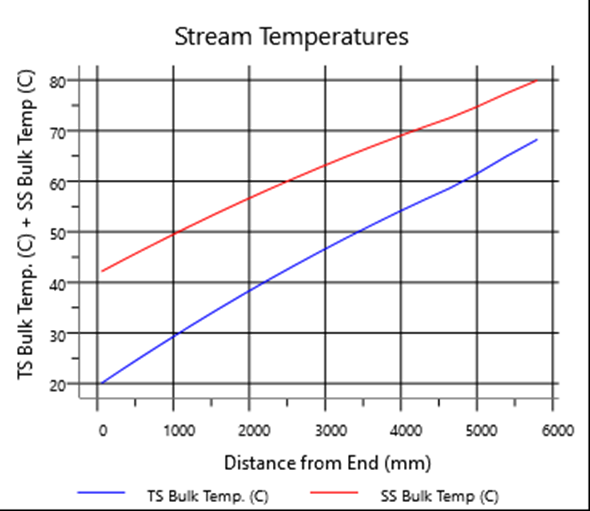
\includegraphics[trim= 0cm 0.1cm 0.1cm 0.5cm, clip, width=\textwidth]{Figures/Proces_Analysis/HX.png}
		\caption{Stream temperatures along the heat exchanger}
	\end{subfigure}
	\hfill
	\begin{subfigure}[b]{0.9\textwidth}
		\centering
		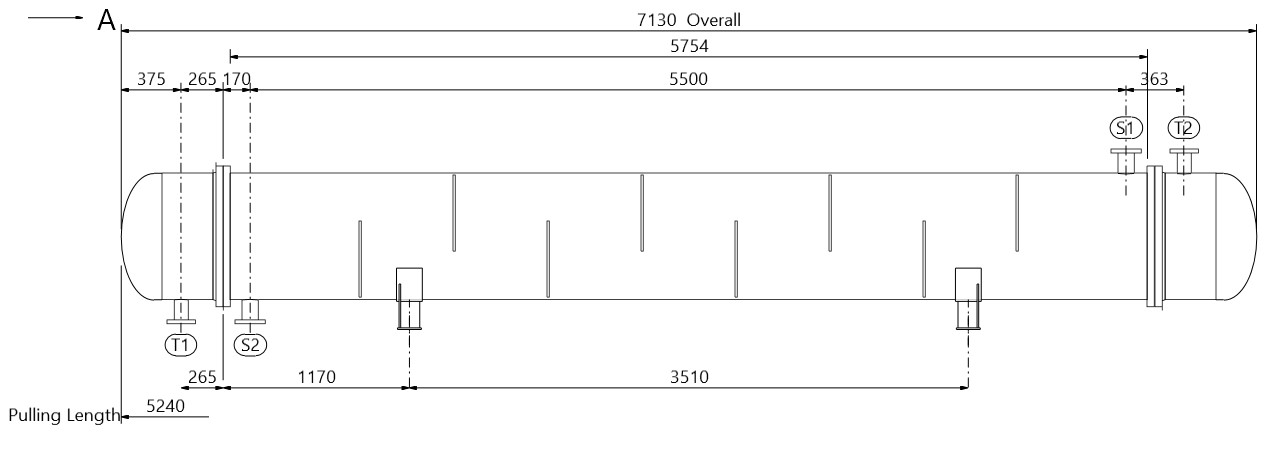
\includegraphics[width=\textwidth]{Figures/Proces_Analysis/HX2.jpg}
		\caption{External dimension of the heat exchanger}
	\end{subfigure}
	\caption{Results of heat exchanger design}
	\label{fig:Ester_HX}
\end{figure}



\section{Sensitivity Analysis}

The \textit{sensitivity analysis} allows evaluating a parameter's influence on model output. In this case, the reactor's diameter and length are selected as degrees of freedom and can be manipulated. The system output is the amount of the methyl lactate at the reactor outlet.

In \textit{Vary} section, two variables are created: one corresponds to the length of the reactor, while the second one is the diameter of the reactor. Both variables are \textit{Block-Var} Type. Let the length change from $1~[m]$ to $100~[m]$ every $1[m]$, and the diameter change from $0.1-1.5~[m]$ every $0.1~[m]$.
In \textit{Define} section, model output is defined. The model output is affected by a change from \textit{Vary} section. The output variable, in this case, is the mole flowrate of methyl lactate in the outlet stream. The mole flowrate can be found in the \textit{Streams} category.

The sensitivity analysis results are in Figure \ref{fig:Ester_Sensitivity_Analysis}.

\begin{figure}[h!]
	\centering
	\begin{subfigure}[b]{0.99\textwidth}
		\centering
		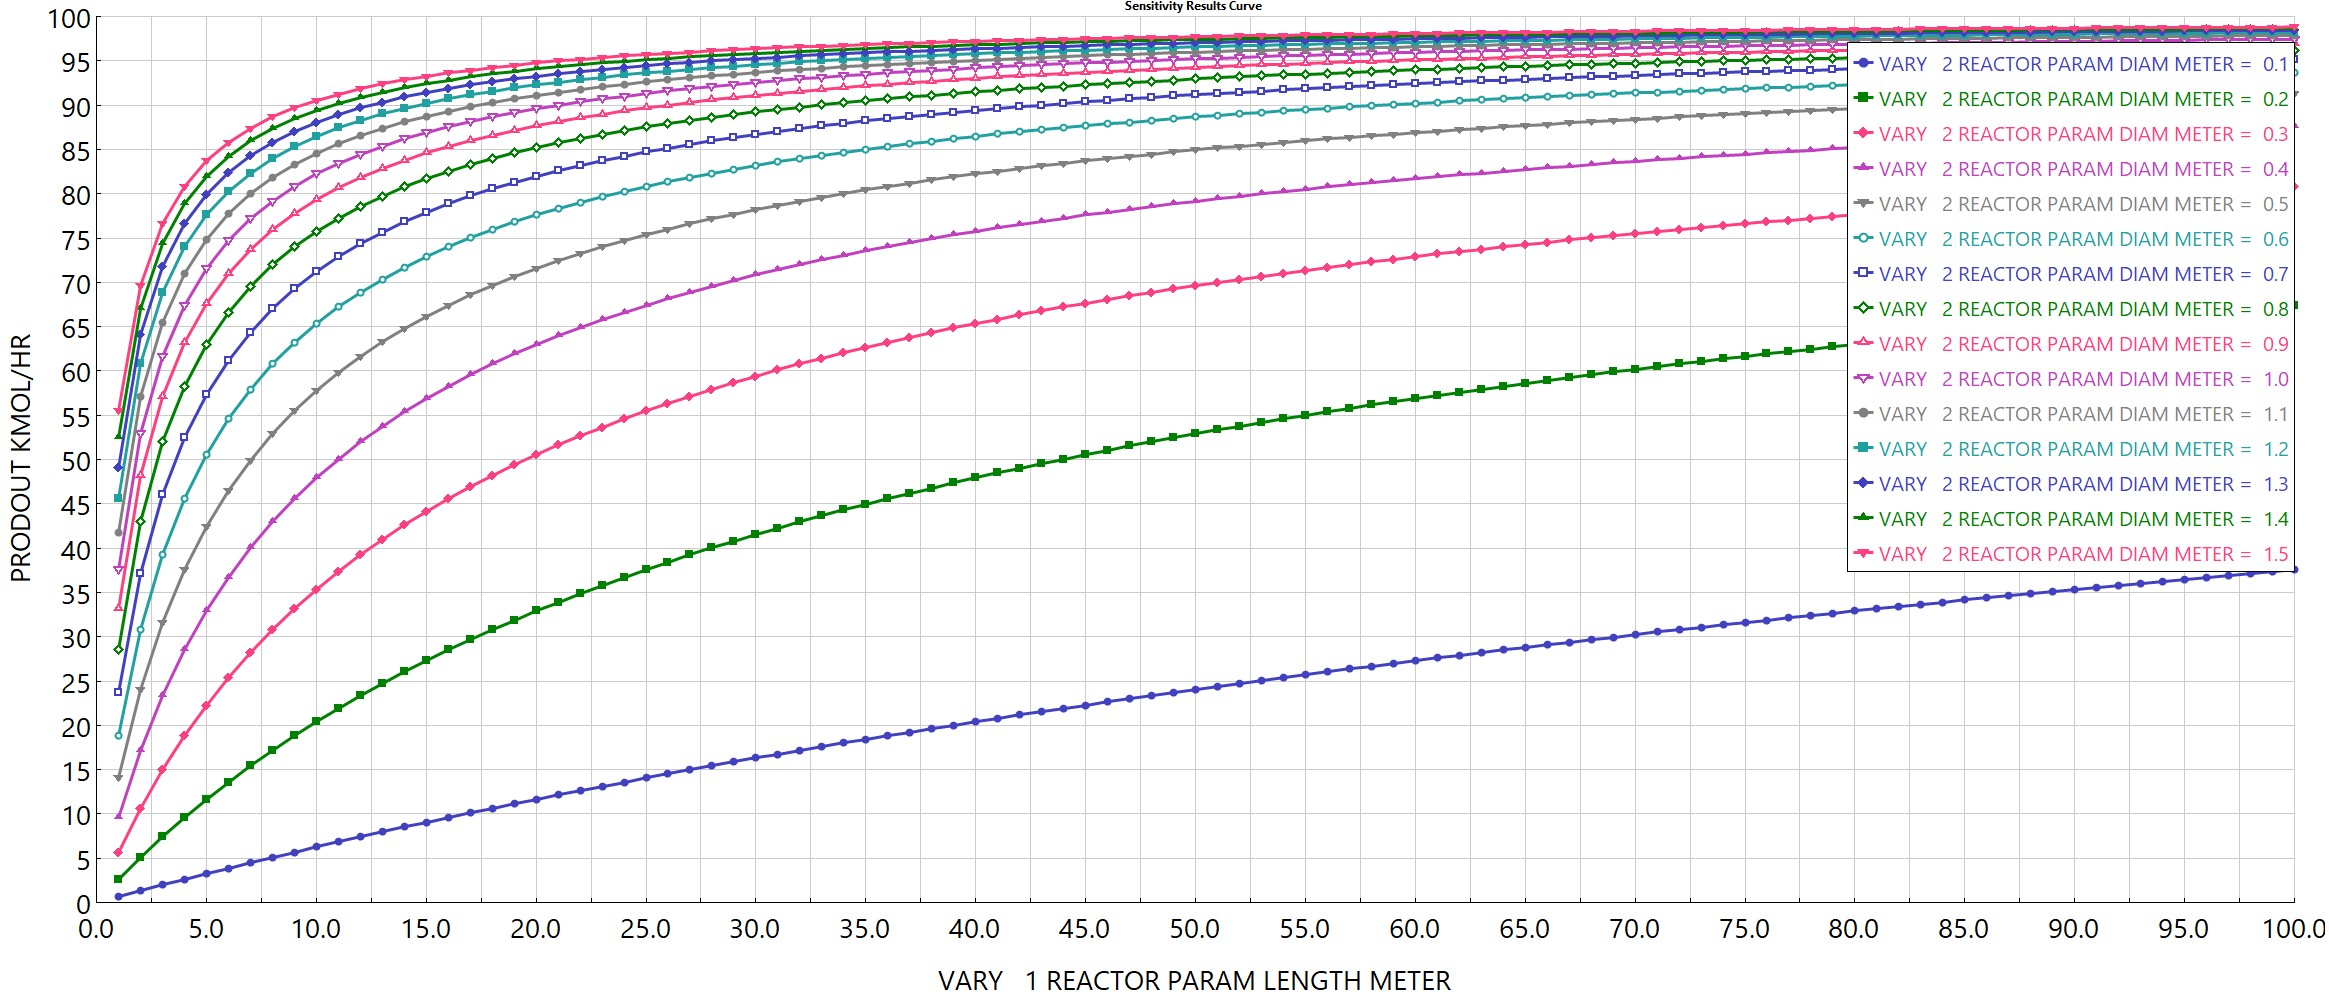
\includegraphics[width=\textwidth]{Figures/Proces_Analysis/Parametric_sensitivity_analysis.jpg}
		\caption{Sensitivity analysis - linear scale}
	\end{subfigure}
	\begin{subfigure}[b]{0.99\textwidth}
		\centering
		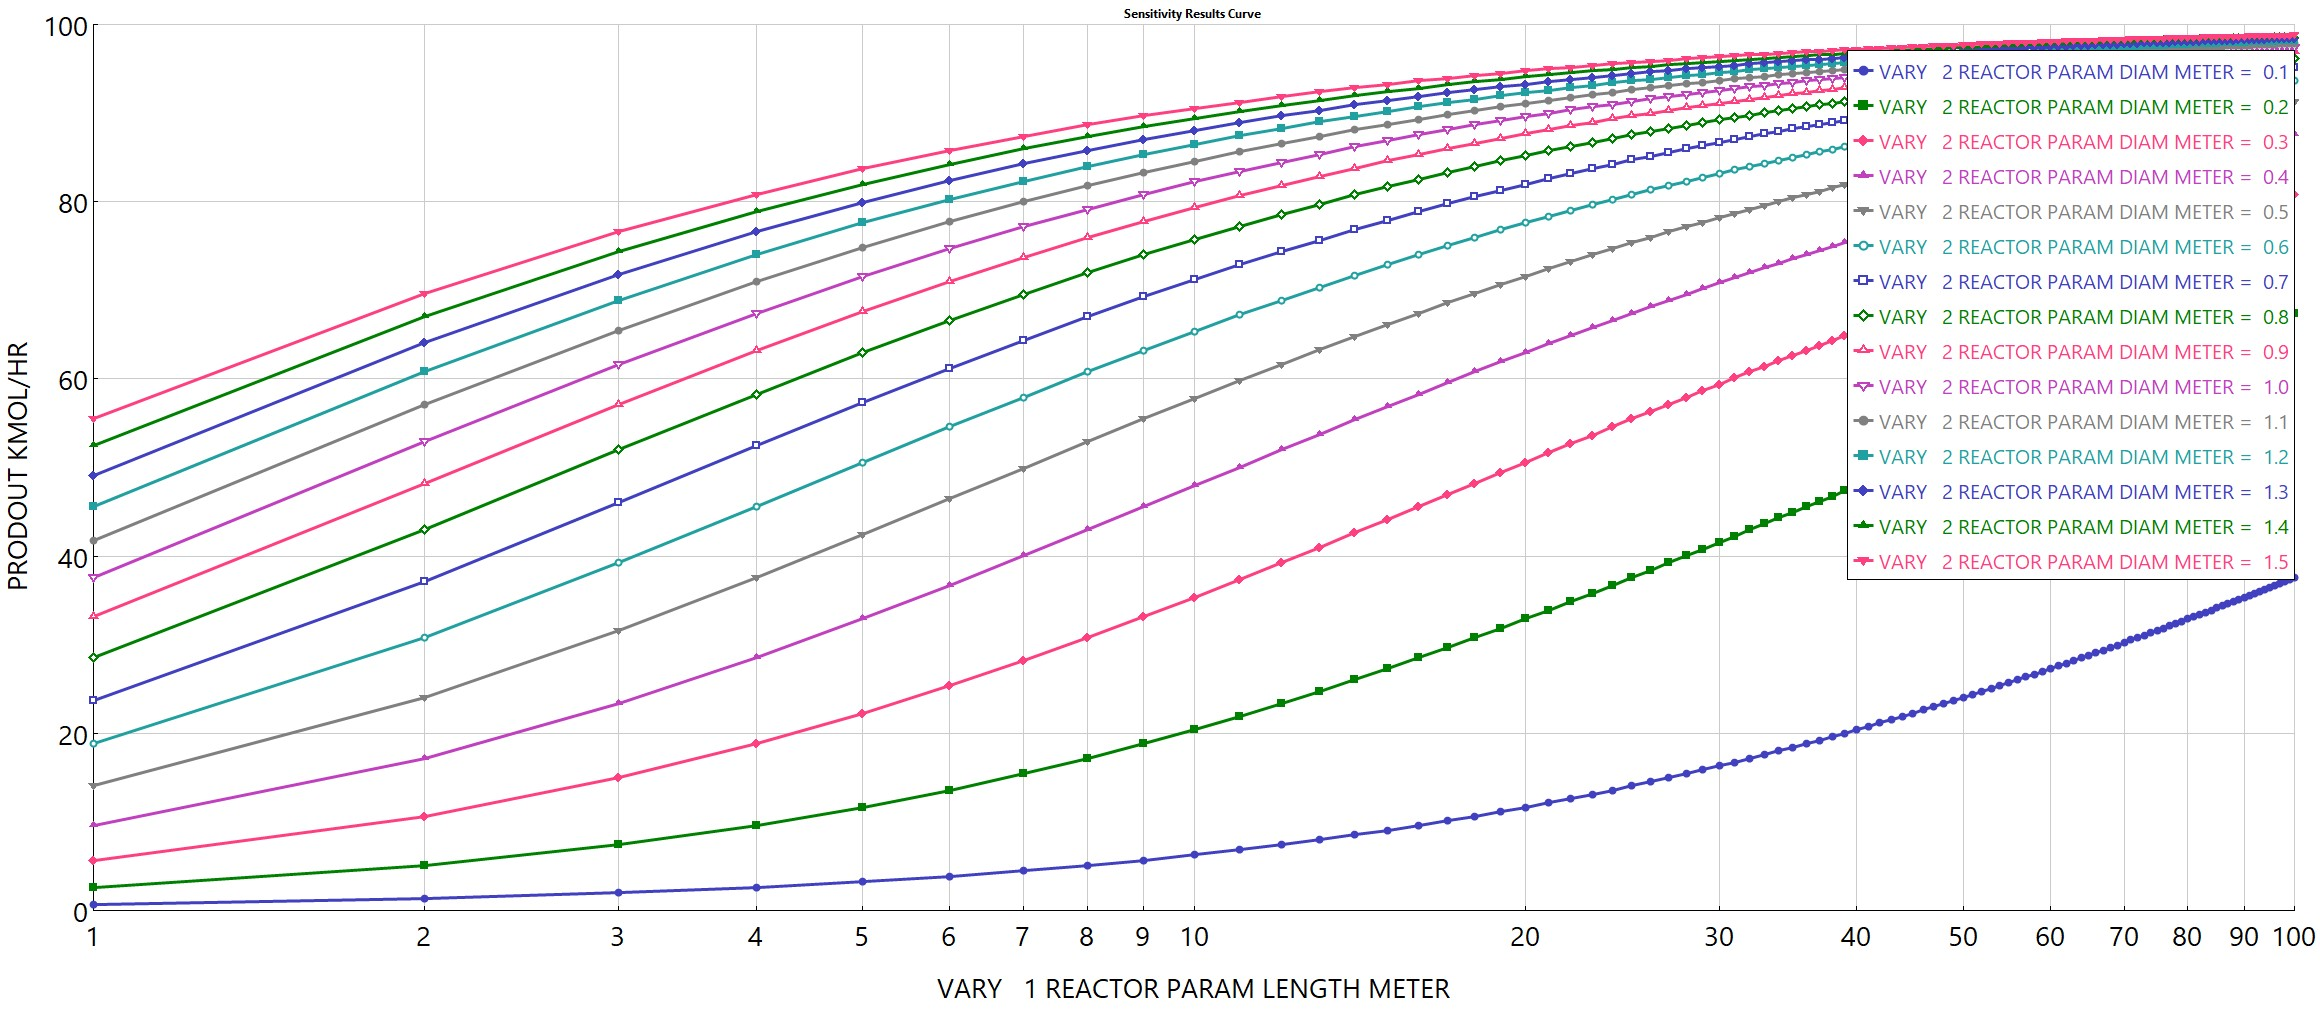
\includegraphics[width=\textwidth]{Figures/Proces_Analysis/Parametric_sensitivity_analysis_inverse.jpg}
		\caption{Sensitivity analysis - log scale}
	\end{subfigure}
	\caption{Sensitivity analysis results}
	\label{fig:Ester_Sensitivity_Analysis}
\end{figure}

As shown in Figure \ref{fig:Ester_Sensitivity_Analysis}, the initial value of reactors length and diameter are insufficient to obtain high conversion.

The next step is defining a local variable describing lactic acid's conversion. Three variables need to be defined in the $Define$ section. Two variables describe the molar flowrate of lactic acid at the inlet and the outlet stream, and the third one describes the conversion rate. The molar flowrates can be found in the \textit{Streams} category. The conversion is defined as \textit{Local-Param}, but the conversion formula should be written in the \textit{Fortran} section. 

Be careful to use the symbols in the exact form as they are defined in the \textit{Define} page. The conversion can be calculated from the following equation:

\begin{equation}
	CON = \frac{\left( FEED - PRODUCT \right)}{FEED} \cdot 100 \%
\end{equation}

The results of the sensitivity analysis conducted with respect to the conversion are presented in Figure \ref{fig:Ester_Sensitivity_Analysis_Conversion}.

\begin{figure}[h!]
	\centering
	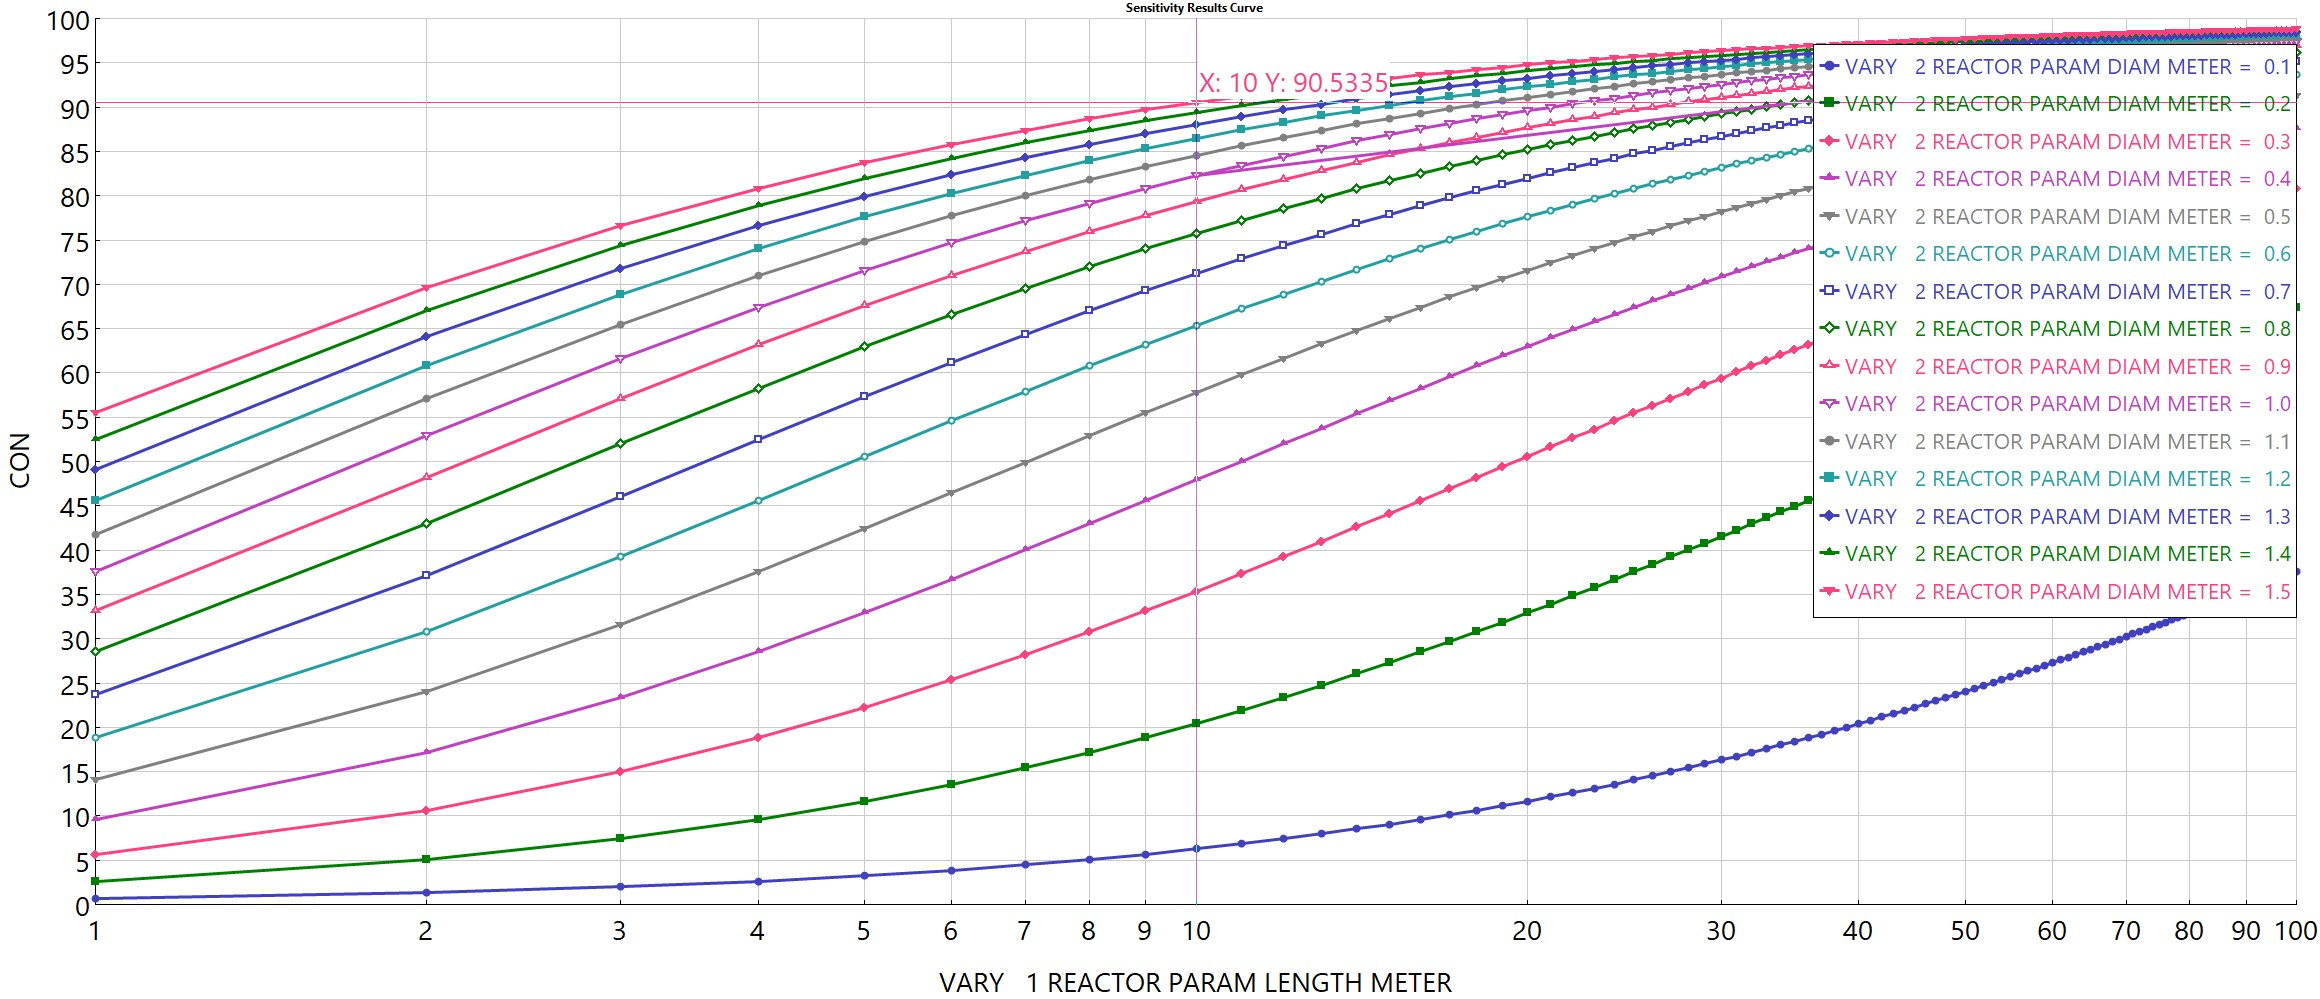
\includegraphics[width=\textwidth]{Figures/Proces_Analysis/Parametric_sensitivity_analysis_conversion.jpg}
	\caption{Sensitivity analysis with respect to conversion}
	\label{fig:Ester_Sensitivity_Analysis_Conversion}
\end{figure}

Based on the sensitivity analysis, we select the first value, which gives us the conversion of 90\%, so the length of $10~[m]$ and the diameter of $1.5~[m]$. Any reasoning can be applied to select the reactor size. One can perform a similar analysis with respect to any indicator and use it to draw a conclusion.

\section{Design-spec}

Let's investigate how to separate compounds of the stream leaving the reactor. By analysing singular points from the Distillation Synthesis Analysis (Table \ref{tab:Distillation_Singular_Points}), it can be noticed that there is one azeotrope.

\begin{table}[h!]
	\centering
	\adjustbox{max width=\textwidth}{%
	\begin{tabular}{l|llllllll}
		& Temp (C) & Classification & Type        & No. Comp. & LACTI-01 & METHA-01 & METHY-01 & WATER \\ \hline
		1 & 216.627  & Stable node    & Homogeneous & 1         & 1.000    & 0.000    & 0.000    & 0.000 \\
		2 & 64.535   & Unstable node  & Homogeneous & 1         & 0.000    & 1.000    & 0.000    & 0.000 \\
		3 & 144.813  & Saddle         & Homogeneous & 1         & 0.000    & 0.000    & 1.000    & 0.000 \\
		4 & 100.018  & Saddle         & Homogeneous & 1         & 0.000    & 0.000    & 0.000    & 1.000 \\
		5 & 99.855   & Saddle         & Homogeneous & 2         & 0.000    & 0.000    & 0.027    & 0.973
	\end{tabular} }
	\caption{Singular points from the Distillation Synthesis Analysis}
	\label{tab:Distillation_Singular_Points}
\end{table}

The same conclusion can be drawn form of the ternary plot (Figure \ref{fig:Ester_Teranry}).

\begin{figure}[H]
	\centering
	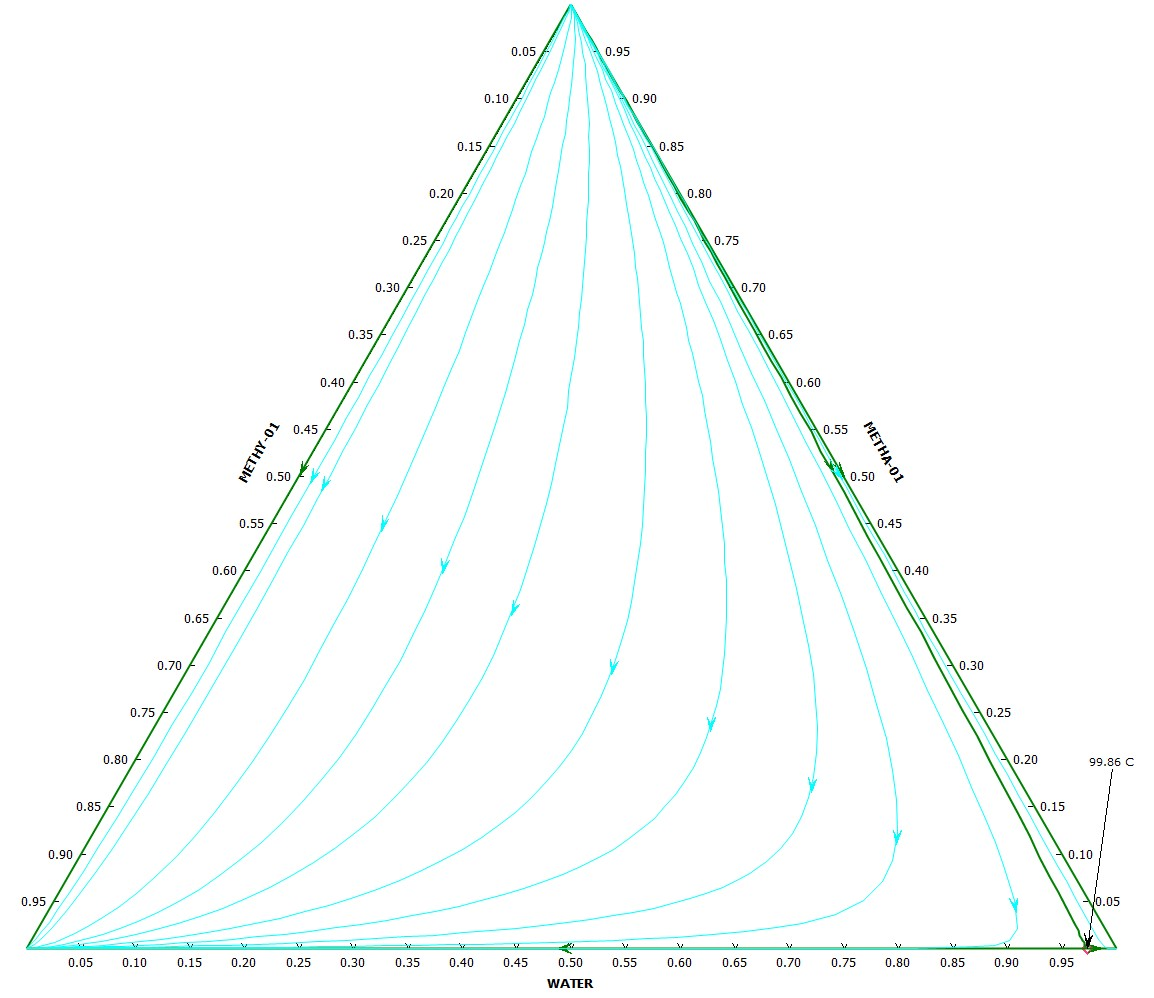
\includegraphics[width=0.5\textwidth]{Figures/Proces_Analysis/Distillation.jpg}
	\caption{Ternary plot}
	\label{fig:Ester_Teranry}
\end{figure}

In this simulation work, we are going to remove non-azeotropic components first. We start with \textit{METHA-01}, one of the reactants with the lowest boiling point. The distillation column is modelled with \textit{RadFrac} module. We assume the number of stages to be 30 and the feed stage to be 15. The distillation column is characterized by the Distillate rate equal to the mole flowrate of the \textit{METHA-01}, and the molar reflux ratio equal to 1.
The \textit{Design-spec} is used to increase the bottom stream's purity. It is assumed that the number of stages, the feed stage and the distillate rate are fixed, but the reflux ratio can be manipulated. The \textit{Design-spec} can be found in the \textit{Flowsheeting Option} folder. First, the model output needs to be defined. In this case, the model output is the mole fraction of acetic acid in the bottom stream. In the \textit{Spec} section, the target value of the model output is specified. We assume that the bottom stream should have the molar fraction of the acetic acid equal to $1e-4$, with tolerance $1e-5$. The next step is to define what parameter can be used to tune the model output. In this case, we used the molar reflux ratio, which can vary from 0.5 to 2. The adjusted value of the reflux ratio is 1.5524972, and simulation results can be found in Table \ref{tab:Col1_results}.

\begin{table}[h!]
	\centering
	\adjustbox{max width=\textwidth}{%
	\begin{tabular}{ll|lll}
					   &         & Product  & Distillate& Bottom  \\ \hline
		Mole Flows     & kmol/hr & 400      & 190.51  	& 209.5    \\
		LACTI-01       & kmol/hr & 9.467    & 9.467   	& 4.82E-50 \\
		METHA-01       & kmol/hr & 209.467  & 0.019		& 209.45   \\
		METHY-01       & kmol/hr & 90.53 	& 90.53		& 2.61E-16 \\
		WATER          & kmol/hr & 90.53 	& 90.48		& 0.053   \\ \hline
		Mole Fractions &         &          &     		&          \\
		LACTI-01       &         & 0.023	& 0.050   	& 2.30E-52 \\
		METHA-01       &         & 0.523	& 0.0001 	& 0.9997    \\
		METHY-01       &         & 0.226	& 0.476  	& 1.2450E-18 \\
		WATER          &         & 0.226	& 0.475   	& 0.000251
	\end{tabular} }
	\caption{Stream results of the distillation column}
	\label{tab:Col1_results}
\end{table}

\section{Column Internals}

The next step is to analyse the distillation column from the hydraulic point of view. The fact that the simulation of the distillation column has converged and satisfies the mass balance doesn't mean that the hydraulics are well designed. This requires special attention and separate analysis. The analysis tools for a column hydraulic can be found in the \textit{Column Internals} folder. One can use the \textit{Auto Section} option to create different sections along the column. In this case, the software suggests two sections of different diameters (both with sieve trays). One section is above, and the second is below the feed stage. The results of the auto-section tool are given in Table \ref{tab:ColHydraulic_auto}.

\begin{table}[h!]
	\adjustbox{max width=\textwidth}{%
	\begin{tabular}{l|llllllllllllllll}
		Name & Start Stage & End Stage & Mode               & Internal Type & Tray/Packing Type & Number of Passes & Tray Spacing/Section Packed Height & Dimension & Diameter    & Dimension \\ \hline
		CS-1 & 2           & 14        & Interactive sizing & Trayed        & SIEVE             & 1                & 0.6096                             & meter     & 1.608  & meter     \\
		CS-2 & 15          & 29        & Interactive sizing & Trayed        & SIEVE             & 1                & 0.6096                             & meter     & 1.596 & meter     
	\end{tabular} }
	\caption{Column design given by automatic tool}
	\label{tab:ColHydraulic_auto}
\end{table}

The graphical representation of the this column is presented on Figure \ref{fig:Ester_Col_hydrarulic_auto}

\begin{figure}[h!]
	\centering
	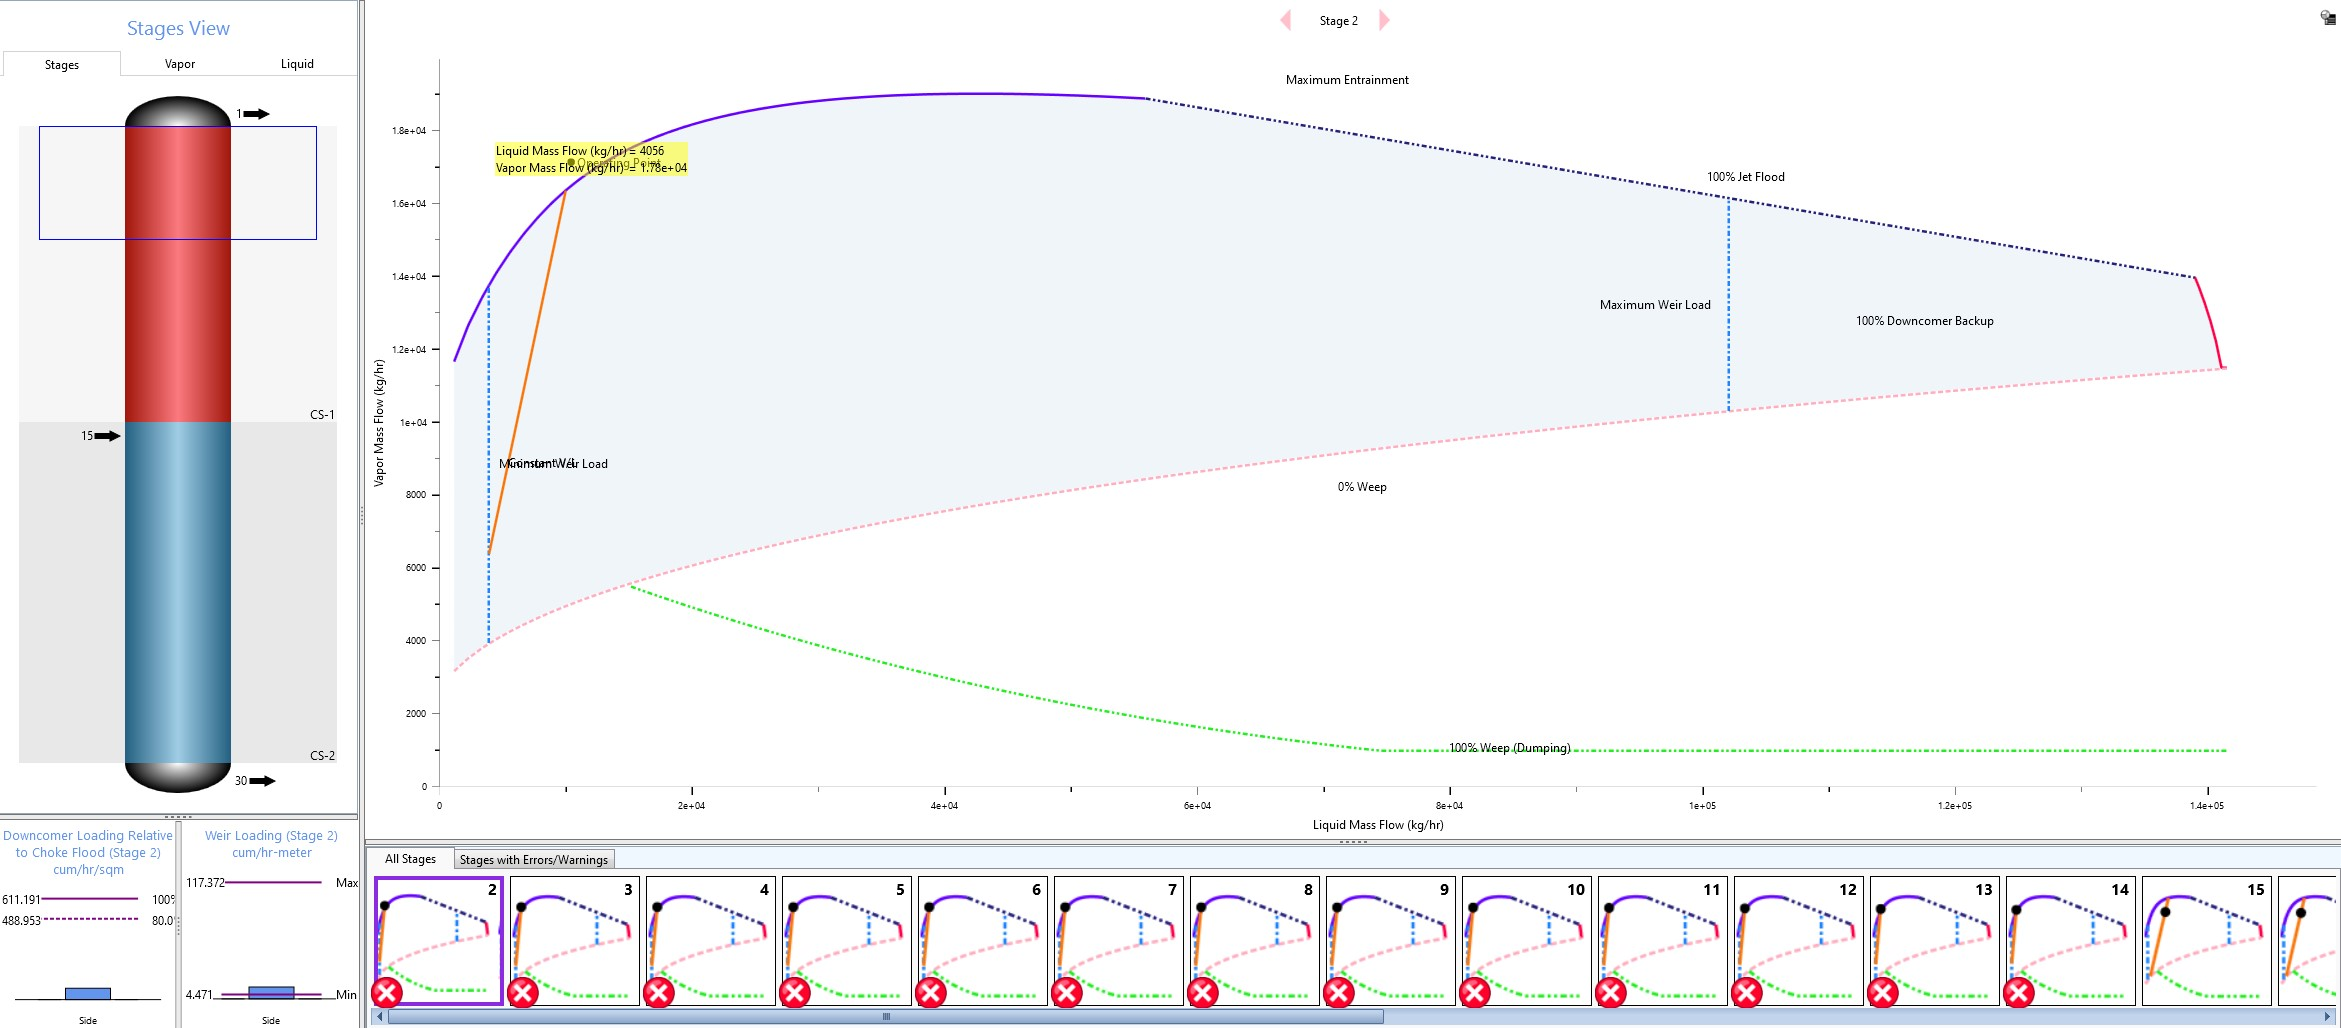
\includegraphics[width=\textwidth]{Figures/Proces_Analysis/Column_Design_Auto.jpg}
	\caption{Column internals}
	\label{fig:Ester_Col_hydrarulic_auto}
\end{figure}

The software returns the following error "Entrainments on Stages 2 - 14 are above the specified maximum percent liquid entrainment of 10. We recommend increasing tray spacing." First, both sections have almost the same diameter (1.6 [m]), so the whole column can be represented by one section. The error given by the software can be solved by increasing the spacing from the default value of 0.6096 [m] to 0.75 [m]. Figure \ref{fig:Ester_Col_hydrarulic_manual} presents the corrected column hydraulic.

\begin{figure}[H]
	\centering
	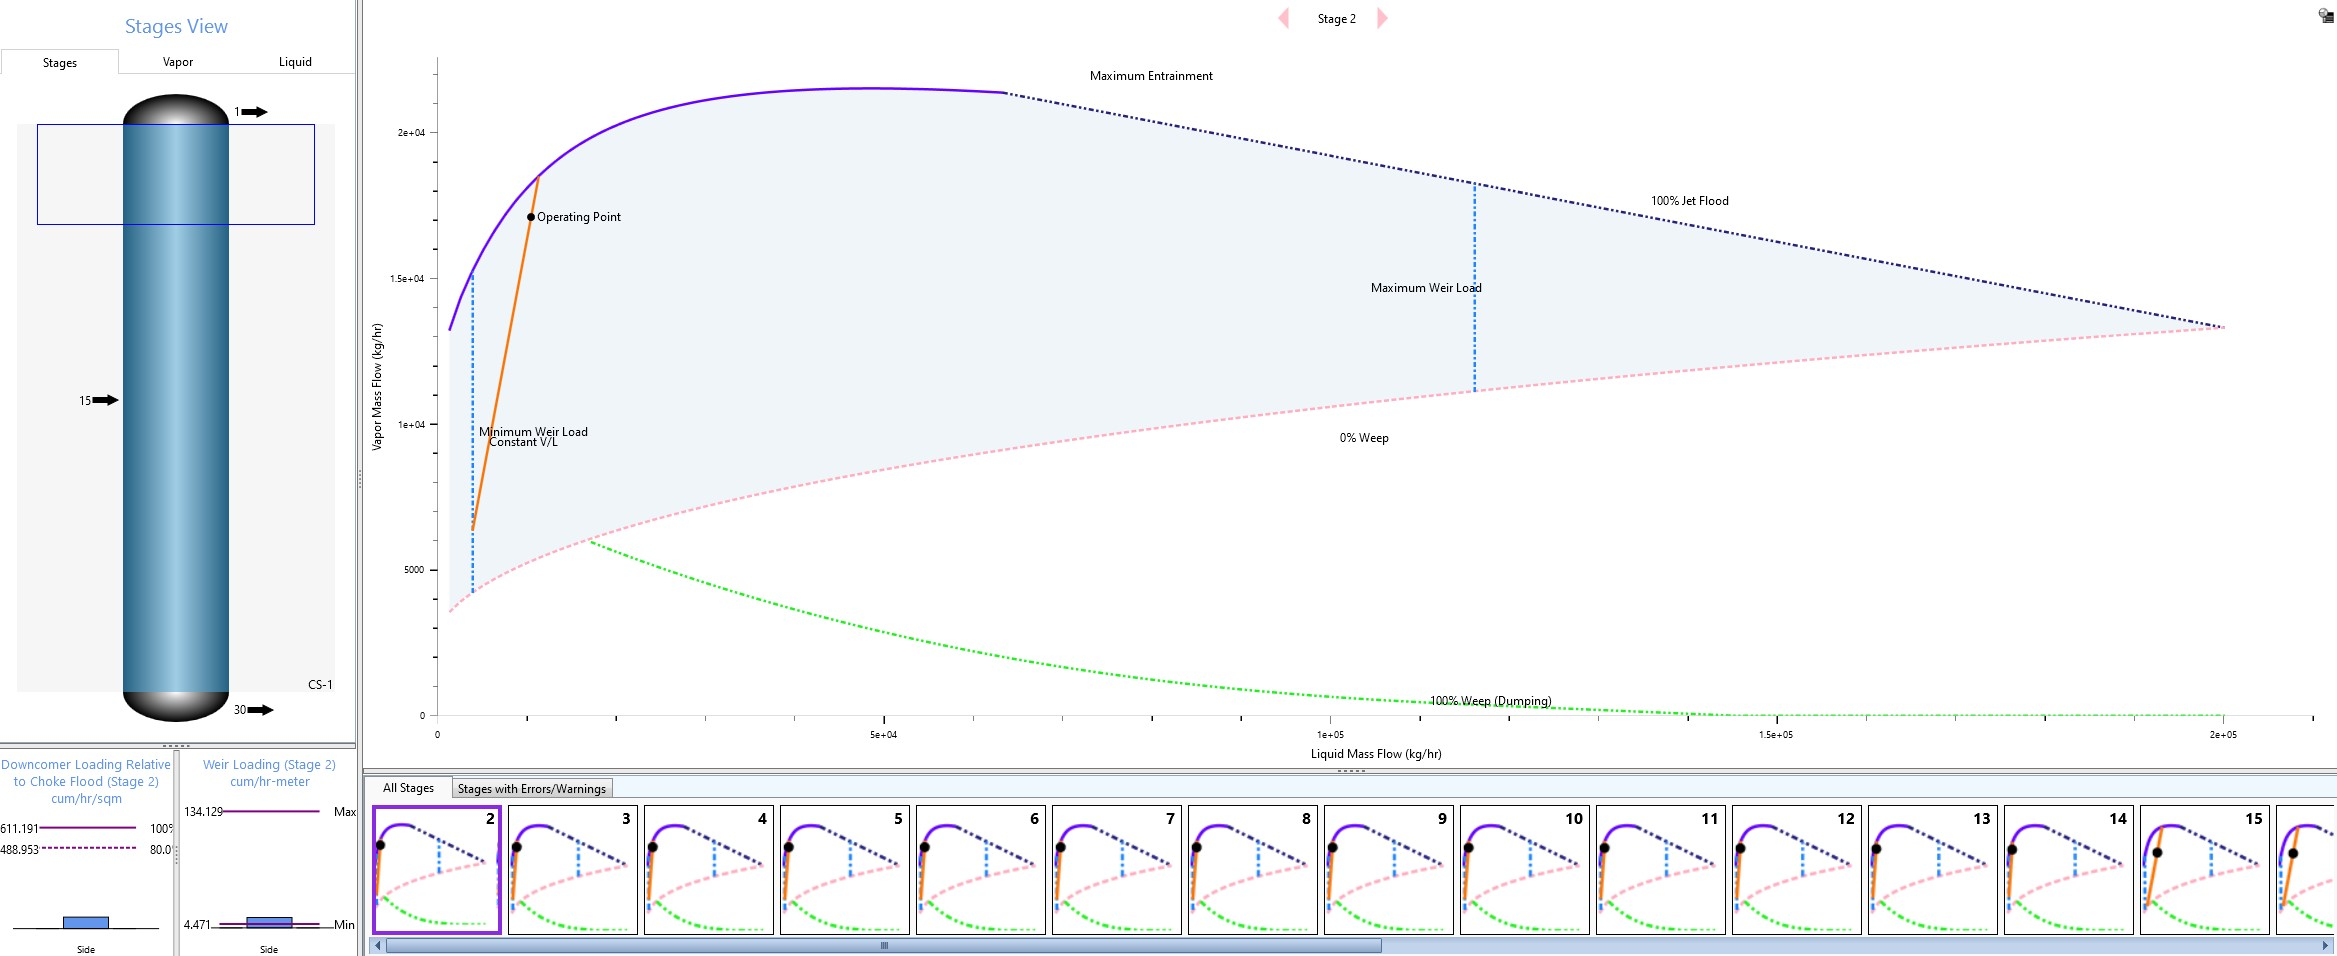
\includegraphics[width=\textwidth]{Figures/Proces_Analysis/Column_Design_Manual.jpg}
	\caption{Column internals}
	\label{fig:Ester_Col_hydrarulic_manual}
\end{figure}






